\documentclass[12pt]{article}
\usepackage[utf8]{inputenc}
\usepackage[margin=1in]{geometry}
\usepackage{times}
\usepackage{multicol}
\usepackage{graphicx}

% Please change the name if you can think of something better
\title{Social Distancing:\\\large The Importance of Staying Isolated While the Nation Begins to Open}
\author{Woloshyn, Christopher\\
\texttt{cwolosh1@binghamton.edu}}

\date{May 2020}

\begin{document}

\maketitle

\begin{abstract}
The goal of this project is to create a comprehensive pandemic simulation that captures the key assumptions of disease spreading and adds its own assumption to model social distancing.
Thousands of simulations will be conducted across a set of differing model parameters; the data this produces will be analyzed and used to inform the best course of action for individuals and governments.
The results from these simulation reveal the importance of reacting early, and reacting strongly.
Governments must be cautious in their endeavors to reopen the economy, but with an informed mindset and proper mitigation infrastructure, can do so without causing a second wave outbreak.
\end{abstract}

\begin{multicols}{2}

\section{Introduction}
As the world enters the next phase of its global pandemic, societies must be ready for the new set of challenges it is going to impose.
For the United States, an important balance between safely reopening the economy, and maintaining strict measures to prevent further outbreaks is, at the time of writing, a top priority.
Unfortunately, as many grow weary of being trapped in their homes unable to work, there may be a misconception between reopening the economy and relaxing social distancing guidelines.
Right now, it is extremely important to evaluate and reinforce the importance of isolation and social distancing.

The goal of this project is to create a comprehensive pandemic simulation that captures some of the key assumptions of disease spreading and social distancing.
Additionally, thousands of simulations will be conducted across a set of differing parameters in the model.
The data this produces will be analyzed and used to inform the best course of action for each individual, and the best course of action for governments.
The results from these simulation will illustrate how to properly mitigate second wave outbreaks while also avoiding new lockdown measures.

\section{Details of the Model}
The model for this project is a rewrite and modification of the source code which was developed by Dr. Hiroki Sayama and his 'SSIE 641: Advanced Topics in Network Science' class on March 11, 2020.
It is built with NetworkX and PyCX Simulator. NetworkX is a Python package used for the creation, manipulation, and study of complex networks.
PyCX Simulator is a simple framework for visualizing time dependent simulations of complex systems.
In this simulation there are two major components.
The first is the actual epidemic model, and the second is the social distancing model that is built on top of the epidemic model.

\subsection{Epidemic Modeling}
The main epidemic model being used is an S.I.R. framework with a Barabási-Albert random network \cite{kermack1927contribution, barabasi1999emergence}. An S.I.R. model stands for \emph{Susceptible, Infected, Recovered}.
This means agents of the simulation can exist in three states: susceptible to getting infected with the disease, infected with the disease, or recovered and therefore immune to the disease.
A Barabási-Albert random network is a network, generated randomly, that follows a scale free distribution.
Most nodes in the network have only a few connections to others, but a few nodes have many connections, and function as hubs.
These types of network models are advantageous because they capture the non-homogeneous nature of social networks.
That is, in traditional epidemic simulations, such as the popular example from the Washington Post \cite{stevens_2020}, every agent in the simulation has roughly the same probability of infection.
However, this is not the case in nature, since some people have more friends than others; those with more friends have a larger list of potentially infected people to encounter.
The Barabási-Albert network captures this.

The simulation begins with a few nodes randomly assigned as initially infected. The probability of a susceptible node becoming infected is constant. For every connection a susceptible node shares with an infected node, the probability of becoming infected the next time step is 20\%. Hence, a node with three infected neighbors has three independent opportunities to become infected, each with probability 0.2.

Every infected node has a chance to recover at any given time step.
This chance increases each time step until 14 days have elapsed in which recovery the next time step is certain.
Every infected node also has a small chance of death on any given time step. A ``dead" node is removed from the network.
In Addition to this death probability, there is also a ``healthcare capacity" parameter that is fixed at 25\% of the population. If there are more infected nodes than there is healthcare capacity, the probability of death increases 4 fold. This is to represent the overwhelming of the healthcare system as observed in other nations such as Italy.

Lastly, there is a system built into this model that tracks the time series data for the number of alive, dead, susceptible, infected, and recovered nodes at each time step. These data will be important for Section \ref{data}. Figure \ref{plots} represents one particular epidemic simulation.
\begin{figure*}[hbt!]
 \centering
 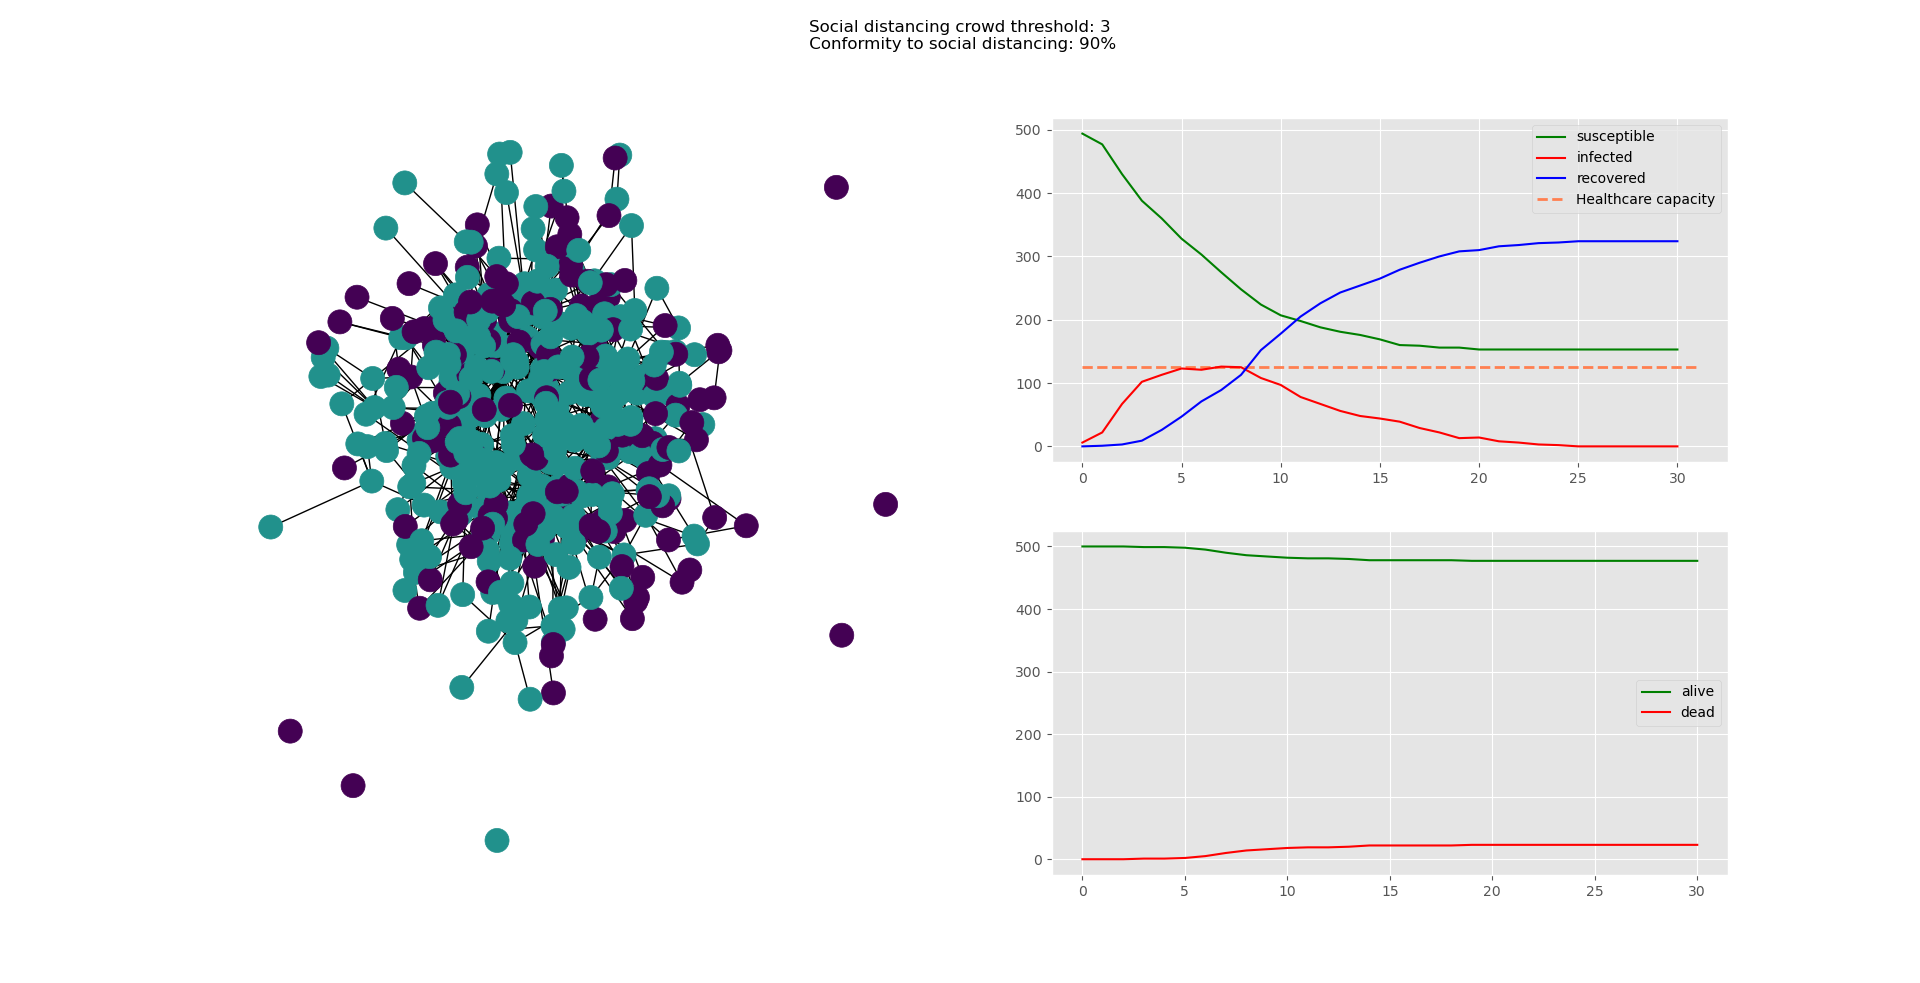
\includegraphics[width=\textwidth]{Figure_1.png}
 \caption{A simulation using a crowd threshold of 3, and 90\% conformity to social distancing.}
 \label{plots}
\end{figure*}

\subsection{Social Distancing Modeling}
The second major component of the model is to capturing the dynamics of social distancing so we can approximate the effects of taking such actions.
There are two adjustable parameters that are embedded in this model.
These will be the two parameters of focus for the large number of simulations.

The first parameter is the ``crowd threshold."
This parameter tells a node when to start social distancing, or lockdowns, etc.
For example, if the crowd threshold is 3, then a particular node will remove all of its connections with neighboring nodes.
Since this isolation condition only depends on neighbors, most infected nodes will likely not remove connection with its neighbors (unless it has a lot of infected neighbors).
This is okay, because it can represent those who are a-symptomatic.
Another interpretation of the crowd threshold is as a ``seriousness" threshold.
If a government takes lockdown action more quickly, then the crowd threshold for the average person is expected to decrease overall.

In addition to the separation mechanics, there are also conditions that cause nodes to re-establish their previously removed connections.
At each time step after isolation, every node has a 10\% chance to reconnect with one of its past neighboring nodes.
This process models the slow, and cautious reformation of social connections.

The second parameter is called ``conformity."
The conformity value represents a probability that a particular node will actually remove a connection between itself and a neighbor. For example, if the conformity value is set to 0.5, then when the crowd threshold is reached, there will be a 50\% chance that the node will remove its connection with a given neighbor.
I.e. 50\% of the time, the node will actually conform and remove that particular connection.
This is meant to model the ``strictness" of social distancing policy, and how seriously it is being taken by the citizens.

\section{Large Scale Data Collection}
\label{data}
Now that the model is in place, and its mechanics have been explained, the next step is to run several thousand independent simulations to account for the randomness that can occur between each simulation.
This way, we can see where the means of those distribution of results falls.

For this experiment, 5 different settings for each of the two social distancing parameters were considered, for a total of 25 different combinations.
For each of these 25 pairs, 1000 simulations of networks containing 5000 nodes were executed for 50 time steps.
The total deaths at the end of the simulation were then assembled into a grid of histograms showing the outcomes depending on the two parameters.

\section{Results}
The results of this experiment were interesting, because they display the effects of both reducing the crowd threshold, and conforming to social distancing guidelines.
Moreover, we can examine the scale of effect between reducing the crowd threshold and increasing social distancing conformity.

To elaborate, both obviously have an effect on the total number of deaths throughout the simulation.
Clearly having the strictest possible guidelines with perfect conformity will lead to the eradication of the disease very quickly, and the total number of deaths near zero.
But what is more interesting is the scale of effect the crowd threshold has over the conformity rate.
For example, in Figure \ref{hist}, when the crowd threshold is 2, we see that conformity only begins to significantly effect the number of deaths when it drops from 60\% to 40\%. 
\begin{figure*}[hbt!]
 \centering
 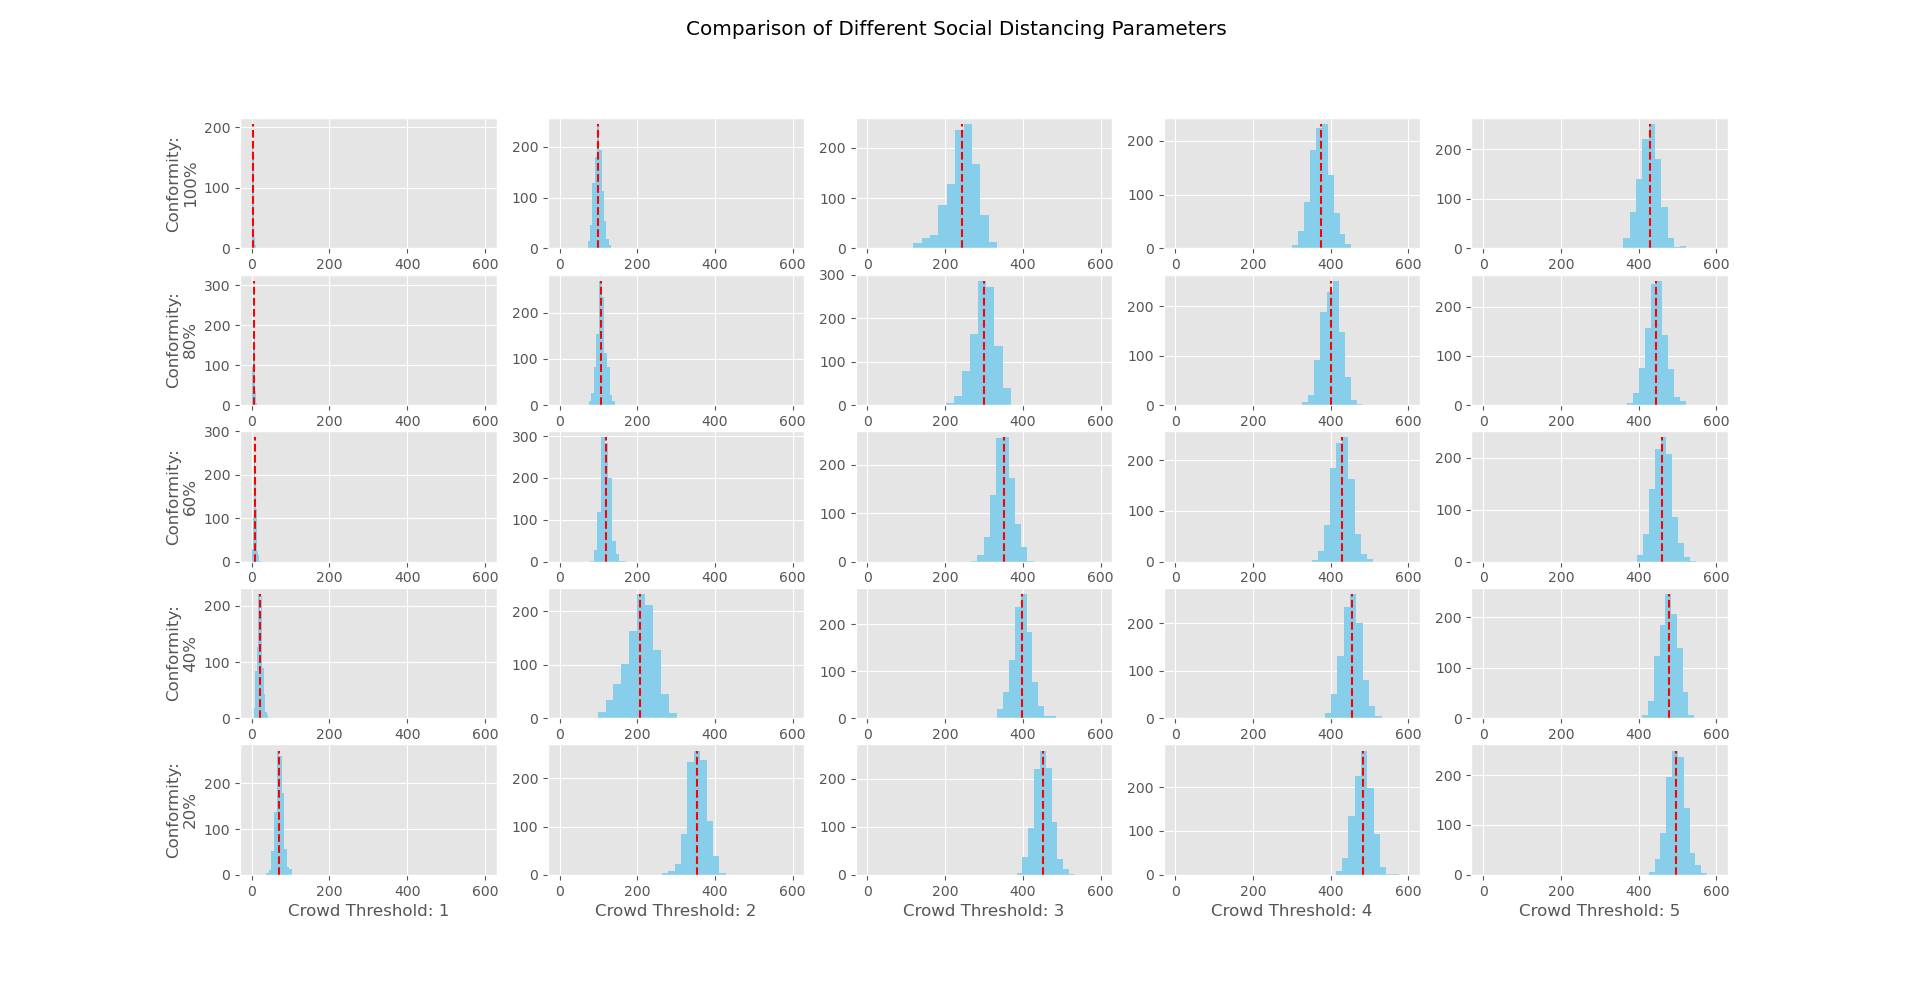
\includegraphics[width=\textwidth]{5000-1000.png}
 \caption{Mortality histograms for 1000 simulations for each of the 25 parameter combinations.}
 \label{hist}
\end{figure*}
Additionally, at crowd threshold 4, the differences between 80\%, 60\%, and 40\% conformity aren't very significant at all.

These are just two examples, but visually we can see that changing from crowd threshold 2 to crowd threshold 3, for instance, has a significant effect on the total number of deaths regardless of the conformity value.
This observation allows us to make a very powerful conclusion.
That is, it is okay if conformity to social distancing is not perfect.
People make mistakes, and people need to go to the store to get supplies, etc.
The biggest impact comes from the recognition of the problem, and the understanding that taking action as early as possible will have the greatest impact.
From this model we learn that the impact of an ``overreaction", with low conformity, is vastly more positive than the impact of an ``under-reaction" that everybody takes seriously.

\section{Conclusions}
With this knowledge, it is essential to keep in mind the importance of maintaining social distancing practices, and it is crucial that governments take the necessary actions to prepare for second waves.
As the United States begins to open up, it must be prepared to recognize the necessity of closing back down, if the situation calls for it.
The insights from this model can help us understand why that is so important.

Conducting even larger simulation with tens of thousands of nodes, and more of them over an extended period of time would be very interesting, although this is more of an issue of time and resources instead of a proposition of future directions.

For future additions to this model, it would be interesting to try and model more closely the reopening process.
Modeling the dynamics of pandemic ``second waves" would offer more direct insight on the exact situation at the time of writing this report.
It could help inform important decisions that are being made right now.

\appendix

\section{Source Code}
All of the code for this project is available on GitHub with the following link:
\newline

\centering
\textbf{https://github.com/cwolosh1/social-distancing}

\bibliographystyle{IEEEtran}
\bibliography{citations}
\end{multicols}

\end{document}